\chapter{MDPs}

What is a decision problem?
Why do we care?

\hypertarget{sequential-decision-problems}{%
\section{Sequential decision
problems}\label{sequential-decision-problems}}

When actions you have taken in the past can bite you in the butt \ldots{}
Maze with pendulums / doors. When moving through the maze, you must
swing the pendulums. In the future you must avoid being hit. (maybe make
a picture of this?) also, is there a more general way to think about it?

% MDPs are a subset of sequential decision problem. Define MDPs. Give
% example.

A MDP is defined as a tuple, \(\{\mathcal S, \mathcal A, P(s_{t+1} \mid s_t, a_t),R(s_t, a_t, s_{t+1}), \gamma\}\)\footnotemark[1]. Where \(s \in \mathcal S\) is the set of possible states (\textit{for example arrangements of chess pieces}), \(a \in \mathcal A\) is the set of actions (\textit{the different possible moves, left, right, diagonal, weird L-shaped thing, ...}),  \(P(s_{t+1} \mid s_t, a_t)\) is the transition function which describes how the environment acts in response to the past (\(s_t\)) and to your actions (\(a_t\)) (\textit{in this case, your opponent's moves, taking one of your pieces, and the results of your actions}), and finally, \(r(s_t, a_t, s_{t+1})\) is the reward function, \textit{whether you won (+1) or lost (-1) the game }.
The objective when solving a MDP is to find a policy, $\pi(a_t | s_t)$, that maximises the discounted cumulative reward, \(R =\sum_{t=0}^T \gamma^t r(s_t, a_t, s_{t+1}) \).

\footnotetext[1]{Why is the discount factor a part of the definition of the MDP?
By defining the discount it ensures the MDP has a unique solution.}

If we wanted we could pick our actions before we make observations,
reducing the search space to only \(|A| \times T\). But this is a bad idea\ldots{} example.

The general feeling of an MDP. - Actions need to be adapted to new
observations and contexts. - While instantaneous results are good, we
care about the longer term aggregates.

\hypertarget{the-markov-property}{%
\subsection{The Markov property}\label{the-markov-property}}

\begin{displayquote}
  What does the M in MDP really mean?
\end{displayquote}

When we say a decision problem is Markovian, we mean that the transition
function generates a Markov chain (ref). The next transition step depends only
on the current state and action. It is invariant to any and all histories that do not
change the current state.

This is not to say that past actions do not effect the future. Rather,
it is a special type of dependence on the past. Where the dependence is
totally described by changes to the \textbf{observable} state.

% Can easily make a sequence Markovian by adding information. E.g.
% time

\hypertarget{optimality}{%
\subsection{Optimality}\label{optimality}}

\begin{displayquote}
  \textit{What does it mean to solve an MDP?}
\end{displayquote}

And importantly, existing theory tells us that there is a unique optima to the bellman iterations.
And that there is always a deterministic policy that is optimal. (usually, there is a unique optima)

(why does this make sense?)


How do we know one policy is better than another? How do we know a
policy is optimal?

\[
\forall \pi\;\; V^{\pi^* } \ge V^{\pi} \\
\]

But, this definition of optimality implicitly assumes a uniform
distribution over states. This is unlikely. Rather, the distribution is
determined by the policy.

\[
\mathop{{\mathbb E}}_{s\sim D_{\pi}} \big[ V^{\pi^* } \big] \ge \mathop{{\mathbb E}}_{s\sim D_{\pi}} \big[ V^{\pi} \big] \\
D_{\pi}(s) = P(s | \pi) = \sum_{\text{all } \tau \text{ with } s_t = s} P(\tau | \pi)
\]

Now. How different is this?

I can imagine some degenerate solutions now being possible? Because we
can control the distribution we are being evaluated on. We could pick a
policy that oscillates between two states, never leaving the cycle.
Therefore it would have \(p(s_1) = p(s_2) = 0.5\) and
\(p(s_{i \neq 1,2}) = 0\).

That doesn't seem so bad?

\begin{displayquote}
  \textit{How hard is it to solve an MDP?}
\end{displayquote}

% Insert lower bound and some intution

\begin{align*}
Q^{\pi}(s_0, a_0) = r(s_0, a_0) &+ \gamma \mathop{\text{max}}_{a_1} \mathop{\mathbb E}_{s_1\sim p(\cdot | s_0, a_0)} \Bigg[ \\
r(s_1, a_1)  &+ \gamma \mathop{\text{max}}_{a_2} \mathop{\mathbb E}_{s_2\sim p(\cdot | s_1, a_1)} \bigg[\\
r(s_2, a_2)  &+ \gamma \mathop{\text{max}}_{a_3} \mathop{\mathbb E}_{s_3\sim p(\cdot | s_2, a_2)} \Big[
\dots \Big] \bigg] \Bigg]
\end{align*}

\hypertarget{how-do-mdps-relate-to-rl}{%
\section{How do MDPs relate to RL?}\label{how-do-mdps-relate-to-rl}}

Reinforcement learning refers to the set of solutions to a type of problem.
This general, reinforcement learning, problem, has two main properties;
\textit{"trial-and-error search and delayed rewards"} \cite{Sutton2018}.
Unlike supervised learning, which gives the learner feedback (\textit{Student: "I think that digit
is a 5". Teacher: "No, it's a 6"}), in RL the learner only receives evaluations (\textit{Student: "I think
that digit is a 5". Teacher: "No."}). This means the student needs to explore the possible answers via some trial-and-error search.
(\textit{Student: "Is it a 4?". Teacher: "No." Student: "How about a 0?". Teacher: "No." ... Student: "A 6?". Teacher: "Yes."})

Ontop of terse teachers, many actions may be taken
before any evaluation is received, thus requiring credit to be assigned to actions,
often leaving the learner wondering: "what did I do to deserve this?" (see
\href{https://www.youtube.com/watch?v=Qv4H81gEGDQ}{pigeon superstition} for an amusing
example of credit assignment gone wrong \cite{Box1997}).

% Your teaher might only give you evaluations for sequences of actions, rather than individual actions.
% Thus you are left with trying to infer how these sequence evaluations tells you about which actions you should take.

The above definition of reinforcement learning is quite general. There are many
different dimensions to problems that have the properties trial-and-error search and
delayed feedback. For example we could make a RL problem that is;

\begin{itemize}
\tightlist
\item
  Observable or un-observable
\item
  Deterministic or stochastic
\item
  Synchronous or asynchronous
\item
  Terminating or infinite
\item
  Discrete versus continuous
\item
  Given knowledge of the underlying model
\end{itemize}

\begin{displayquote}
  But, which setting should we study?
\end{displayquote}

% MDPs are also within the fields of Operational Research, Optimal Control, Mathematical
% Optimisation, Stochastic Programming.


\section{The simplest RL setting}

\begin{displayquote}
  \textit{What is the simplest setting we can consider that still poses an
  interesting challenge to the ML and / or RL communities?}
\end{displayquote}

\hypertarget{a-tabular-representation-of-mdps}{%
\subsection{A tabular representation of MDPs}\label{a-tabular-representation-of-mdps}}

Imagine a tabular MDP, where we can describe the MDP with tables.
A table of three dimensions can describe the transition probabilities, $P[s_{t+1}, s_t, a_t]$,
and a table of two dimensions can describe the rewards, $r[s_t, a_t]$: the states and actions
act as indexes to locations in the tables.

Consider a tabular MDP with deterministic actions, where $P(s_{t+1}|s_t, a_t) \in \{ 0, 1\}$.
This RL problem can be efficiently solved by non-statistical
methods: dynamic programming and related planning techniques \cite{Bertsekas1995}.

But, a tabular MDP with stochastic actions, $P(s_{t+1}|s_t, a_t) \in [0, 1]$,
seems to retain much of the complexity we care about. This setting does not allow
efficient solutions via dynamic programming. And can be approached with algorithms
that are used for state-of-the-art DRL such as policy gradients,

Let's more formally define our tabular MDP.

\begin{align}
\mathcal M &= \{S, A, P, r, \gamma\} \\
S &= [0:n-1] \\
A &= [0:m-1] \\
P &\in [0,1]^{n\times n \times m}, \;\;\forall j, k : \sum_i P[i, j, k] = 1 \\
r &\in \mathbb R^{n\times m}
\end{align}

A result of this formulation is that we consisely write and solve the Bellman equation analytically.

\begin{align}
V &= r_{\pi} + \gamma P_{\pi} V \tag{the bellman eqn}\\
V - \gamma P_{\pi} V &= r_{\pi}\\
(I-\gamma P_{\pi})V &= r_{\pi}\\
V &= (I-\gamma P_{\pi})^{-1}r_{\pi}
\end{align}

The values are written as a vector, $V \in \mathbb R^n$.
The reward under a given policy is written $r_{\pi}[s, a] = \pi[s, a] r[s, a]$.
And the transitions under a given policy is written $P_{\pi}[s', s] = \sum_a P[s', s, a]\pi[s, a]$.


\subsection{The value function polytope}

The value function polytope \cite{Dadashi2018} is the


Imagine a two state MDP. Following some initial, ill-informed policy,
the value that you might get starting from either state state is $v_1, v_2$.



\begin{figure}
\centering

\includegraphics[width=1\textwidth,height=0.25\textheight]{../../pictures/drawings/2-state-automata.png}
\caption{Consider the simplest possible MDP, with two states and two actions. (Any simpler setting is entierly uninteresting. A single state means actions do nothing.
And a single action means all policies are the same...).}
\end{figure}


% \begin{figure}
% \centering
% 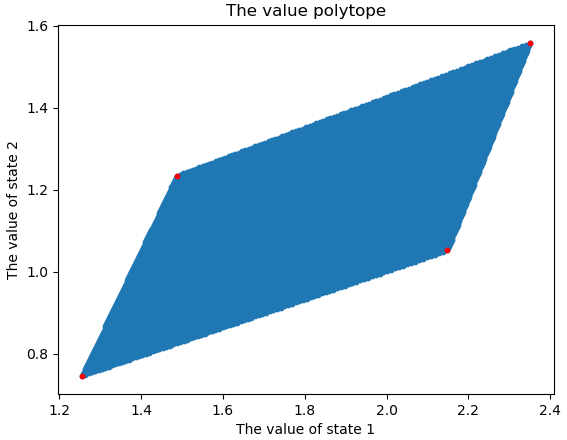
\includegraphics[width=1\textwidth,height=0.25\textheight]{../../pictures/drawings/value-polytope.png}
% \caption{The value polytope for a two state, two action MDP.}
% \end{figure}
